\chapter{Proof for rank 5}

\section{Basic results v2}

\begin{proposition}
  If a vertex is linked with three edges that does not share the other end, then two of those three edges are part of an alternating square.
\end{proposition}

\begin{proof}
  Among the three edges, at least two are not adjacent and thus, they need to be part of an alternating square.
\end{proof}

\begin{corollary}
  If an vertex is not part of any alternating square, then it it connected to at most two other vertices.
\end{corollary}

\begin{proposition}
  In a connected CPR graph over more than two vertices, there no triple edge outside of an alternating square and there is no double edge such that the difference between indices is not 2.
\end{proposition}

\begin{proof}
  Each end of the triple edge is not part of an alternating square and so must not be connected to more than 2 vertices. But the graph is connected, so at least one end of the graph must be connected to more than one vertex. So one end must be connected to two vertices but then the edge that connect this vertex to the new one must be adjacent to all three edges. But that is impossible.
\end{proof}

\begin{proposition}
  An alternating square can be connected to a simple edge (no part of an alternating square) only if it have two adjacent simple edges with a difference in indices of exactly 2.
\end{proposition}



\section{Basic results}

\paragraph{}
Dans la suite, nous noterons les carrés alternés grâce au deux involutions qui les composent. Un carré alterné avec des arêtes $\rho_0$ et $\rho_2$ sera noté $[\rho_0, \rho_2]$.

\begin{definition}
  Deux carrés alternés sont dit adjacents s'ils partagent deux sommets\footnote{Ces définitions sont à améliorer, il y a quelques problèmes mais je pense qu'il y a moyen de rendre ça correct}.
\end{definition}

\begin{definition}
  Une suite de carrés alternés adjacents est un suite finie dans laquelle chaque carré alterné est adjacent avec son précédesseur et son successeur s'ils existent.
\end{definition}

\begin{definition}
  Une suite de carré alternés adjacents est dite linéaire si une des deux composante de sa notation est constante.
\end{definition}

Par exemple, la suite $[\rho_0, \rho_2], [\rho_0, \rho_4], [\rho_0, \rho_3]$ est linéaire car la première composante est toujours $\rho_0$.

\begin{definition}
  Une suite de carré alterné est dite monotone si la suite formée par les différences des indices de ses carrés est monotone.
\end{definition}

La suite $[\rho_0, \rho_2], [\rho_0, \rho_3], [\rho_0, \rho_4]$ est monotone, en effet la suite formée par la différente des indice est $2, 3, 4$ et cette suite est bien monotone.

\begin{proposition}
  Toute suite de carrés alternés monotone est linéaire.
\end{proposition}

\begin{proof}
  Une suite monotone non-linéaire serait de la forme suivante: $[\rho_{i-1}, \rho_j], [\rho_i, \rho_j], [\rho_i, \rho_{j+1}]$, si nous représentons le graphe d'une telle suite nous obtenons le graphe suivant:

  \begin{figure}[H]
    \begin{center}
      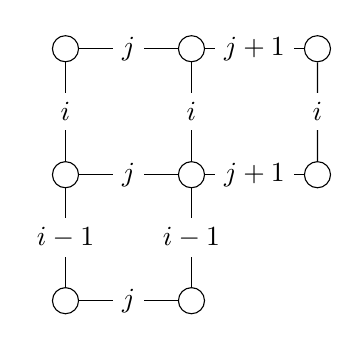
\begin{tikzpicture}[scale=.8]

        \begin{scope}[every node/.style={circle,draw}]
          \node (1)  at (0,2)  {};
          \node (2)  at (0,0)  {};
          \node (3)  at (0,-2) {};
          \node (4)  at (2,2)  {};
          \node (5)  at (2,0)  {};
          \node (6)  at (2,-2) {};
          \node (7)  at (4,2)  {};
          \node (8)  at (4,0)  {};
        \end{scope}

        \begin{scope}[every node/.style={fill=white}]

          \begin{scope}[every edge/.style={draw}]
            \path (2)  edge node {$i-1$} (3);
            \path (5)  edge node {$i-1$} (6);
            \path (1)  edge node {$i$} (2);
            \path (4)  edge node {$i$} (5);
            \path (7)  edge node {$i$} (8);
            \path (1)  edge node {$j$} (4);
            \path (2)  edge node {$j$} (5);
            \path (3)  edge node {$j$} (6);
            \path (4)  edge node {$j+1$} (7);
            \path (5)  edge node {$j+1$} (8);
          \end{scope}
        \end{scope}

      \end{tikzpicture}
      \caption{Suite de carrés alternés monotone et non-linéaire}
    \end{center}
  \end{figure}

  \paragraph{}
  Nous avons un problème en bas à droite, nous ne pouvons pas ajouter de carré à cet endroit sinon nous n'avons plus une suite, donc il faut que $i-1$ et $j+1$ soit consécutifs. On a alors $i = j+1$ ou $i+1=j$ étant donné la symétrie nous pouvons n'en conserver qu'une. Prenons $i = j+1$, ceci est un problème car alors notre carré alterné $[\rho_i, \rho_j]$ n'en est plus un, en effet $|i-j| = 1$.

\end{proof}

\begin{lemma}
  La parité de la taille d'une suite de carrés alternés est toujours la même que la partité d'une suite monotone qui admet les deux même extrémités.
\end{lemma}

\begin{lemma}
  \label{lemma-continue-alternating-square}
  Si on a un carré alterné dont les indices différent de plus 2 alors le seul moyen de l'étendre est d'utiliser un autre carré alterné.
\end{lemma}

\begin{corollary}
  Si nous travaillons sur un nombre impair de points et si nous avons un carré alterné dont la différence des indices est de plus de 2, alors toute extension de ce carré alterné à tous les points contient une suite de carrés alternés qui comprend un carré dont la différence des indices est exactement 2.
\end{corollary}

\begin{proof}
  Chaque fois que nous étendons avec un carré alterné nous ajoutons deux points. Si nous avons un nombre impair de points alors nous ne pouvons pas utiliser que des carrés alternés pour les relier. Mais si nous avons un carré alterné dont la différence des indices est de plus de deux, nous devons forcément l'étendre à un autre carré alterné. Et ainsi de suite jusqu'à avoir tous les points ou à arriver à un carré alterné dont la différence des indice ne vaut plus que deux. Le premier cas est impossible donc c'est forcément le second qui arriver.
\end{proof}

\begin{lemma}
  La taille d'une suite monotone partant du carré alterné $[i, j]$ et arrivant à une carré donc la différence des indices est 2 est $|i - j| - 2$.
\end{lemma}

\begin{lemma}
  Une arête double dont la différence des indices est supérieure à 2 ne peut être relié que par un carré alterné.
\end{lemma}

\section{Intermediate results}

\begin{lemma}
  \label{lemma-forbidden-alternating-square}
  Let $\Gamma$ be sggi generating $A_{11}$ of rank 5. Then its permutation representation graph does not contains an alternating square between $\rho_0$ and $\rho_4$ if $\rho_0$ is a 4-transposition\footnote{Is this condition necessaraly?}.
\end{lemma}

\begin{proof}
  This proof and the following ones will use the same ideas to try to build valid permutation representatioin graph
  \begin{itemize}
    \item First, a pattern will be choosen and placed it on the graph (in this case, it's an alternating squre between $\rho_0$ and $\rho_4)$
    \item Then all mandatory edges will added such that the pattern can be linked to the rest of the graph
    \item All possibilities to link all the remaining points of the rest of the graph will then be tested
    \item The remaining edges will be eventually placed on the graph such that all involutions are even.
  \end{itemize}

  \paragraph{}
  If no graph were found, that mean that the pattern which has been choosen was impossible. Otherwise, this method provides a complete list of all graphs.

  \paragraph{}
  Let's start by placing the 4-transposition $\rho_4$ on the graph. We have the following graph:

  \begin{figure}[H]
    \begin{center}
      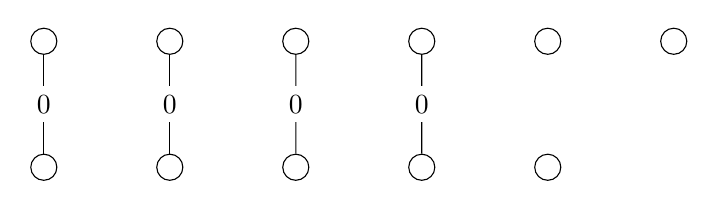
\begin{tikzpicture}[scale=.8]

        \begin{scope}[every node/.style={circle,draw}]
          \node (1)  at (0,2)  {};
          \node (2)  at (0,0)  {};
          \node (3)  at (2,2)  {};
          \node (4)  at (2,0)  {};
          \node (5)  at (4,2)  {};
          \node (6)  at (4,0)  {};
          \node (7)  at (6,2)  {};
          \node (8)  at (6,0)  {};
          \node (9)  at (8,2)  {};
          \node (10) at (8,0)  {};
          \node (11) at (10,2) {};
        \end{scope}

        \begin{scope}[every node/.style={fill=white}]

          \begin{scope}[every edge/.style={draw}]
            \path (1)  edge node {$0$} (2);
            \path (3)  edge node {$0$} (4);
            \path (5)  edge node {$0$} (6);
            \path (7)  edge node {$0$} (8);
          \end{scope}
        \end{scope}

      \end{tikzpicture}
      \caption{$\rho_0$ est une 4-transposition}
    \end{center}
  \end{figure}

  \paragraph{}
  Now, let's form an alternation square between $\rho_0$ and $\rho_4$.

  \begin{figure}[H]
    \begin{center}
      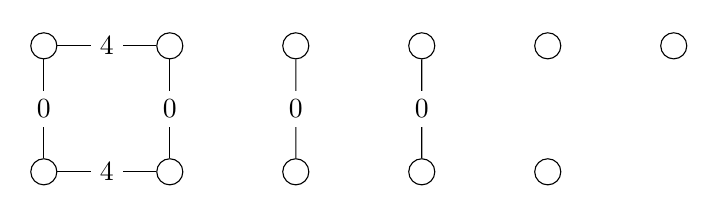
\begin{tikzpicture}[scale=.8]

        \begin{scope}[every node/.style={circle,draw}]
          \node (1)  at (0,2)  {};
          \node (2)  at (0,0)  {};
          \node (3)  at (2,2)  {};
          \node (4)  at (2,0)  {};
          \node (5)  at (4,2)  {};
          \node (6)  at (4,0)  {};
          \node (7)  at (6,2)  {};
          \node (8)  at (6,0)  {};
          \node (9)  at (8,2)  {};
          \node (10) at (8,0)  {};
          \node (11) at (10,2) {};
        \end{scope}

        \begin{scope}[every node/.style={fill=white}]

          \begin{scope}[every edge/.style={draw}]
            \path (1)  edge node {$0$} (2);
            \path (3)  edge node {$0$} (4);
            \path (5)  edge node {$0$} (6);
            \path (7)  edge node {$0$} (8);
            \path (1)  edge node {$4$} (3);
            \path (2)  edge node {$4$} (4);
          \end{scope}
        \end{scope}

      \end{tikzpicture}
      \caption{Cas 1: carré alterné}
    \end{center}
  \end{figure}

  \paragraph{}
  By Lemma~\ref{lemma-continue-alternating-square}, we need to find one sequence of alternating squares until the difference between indices is two. Therefore this sequence contains at least 3 squares. It's impossible to have 5 squares because we only have 11 points. So the sequence is monotone and so linear.

  \paragraph{}
  From the square $[\rho_0, \rho_4]$, we can go to the square $[\rho_1, \rho_4]$ or to the square $[\rho_0, \rho_3]$. But we must use the edges of involution $\rho_0$ now, the two remaining $\rho_0$ edges use 4 points and the sequence of three squares uses 8 points thus they must share at least one point. But no $\rho_0$ edge can be connected to the sequence of alternating square because an $[\rho_{-1}, \rho_1]$ square will be needed to do this but $\rho_{-1}$ does not exist. We cannot use them later in the sequence of alternating square because it is monotone and so, it will never go back to $\rho_0$ once it leave it. The only solution is that the sequence of alternating square must used a $\rho_0$ edge in the next square. The following square in the sequence is therefore $[\rho_0, \rho_3]$.

  \paragraph{}
  Because the sequence is linear, the following square must be $[\rho_0, \rho_2]$. It's the third square and the difference between indices is only two, so we can stop here. For now we have the following graph:


  \begin{figure}[H]
    \begin{center}
      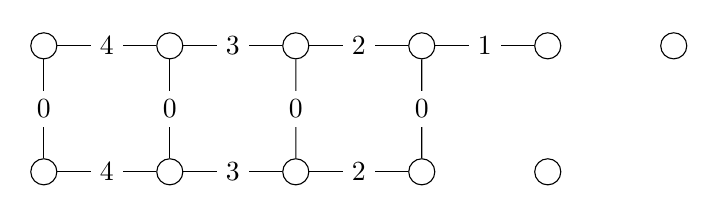
\begin{tikzpicture}[scale=.8]

        \begin{scope}[every node/.style={circle,draw}]
          \node (1)  at (0,2)  {};
          \node (2)  at (0,0)  {};
          \node (3)  at (2,2)  {};
          \node (4)  at (2,0)  {};
          \node (5)  at (4,2)  {};
          \node (6)  at (4,0)  {};
          \node (7)  at (6,2)  {};
          \node (8)  at (6,0)  {};
          \node (9)  at (8,2)  {};
          \node (10) at (8,0)  {};
          \node (11) at (10,2) {};
        \end{scope}

        \begin{scope}[every node/.style={fill=white}]

          \begin{scope}[every edge/.style={draw}]
            \path (1)  edge node {$0$} (2);
            \path (3)  edge node {$0$} (4);
            \path (5)  edge node {$0$} (6);
            \path (7)  edge node {$0$} (8);
            \path (7)  edge node {$1$} (9);
            \path (5)  edge node {$2$} (7);
            \path (6)  edge node {$2$} (8);
            \path (3)  edge node {$3$} (5);
            \path (4)  edge node {$3$} (6);
            \path (1)  edge node {$4$} (3);
            \path (2)  edge node {$4$} (4);
          \end{scope}
        \end{scope}

      \end{tikzpicture}
      \caption{Cas 1.1: doubles carrés alternés}
    \end{center}
  \end{figure}

  \paragraph{}
  To link the two remaining points, we only need two edges but the total amount of edge will be odd but that is fordidden because we want that the generated group is $A_{11}$. To restore parity we need to create a double edge or an alternating square. The number of points if insufficient to create an alternating square, so we must create a double edge and the difference between its indices must be two. All $\rho_0$ edges have already be used, so the possibilities for double edges are $(\rho_1, \rho_3)$ and $(\rho_2, \rho_4)$ but then the number of $\rho_3$ or $\rho_4$ edge becomes odd. So it is impossible to connect all points if $\rho_0$ is a 4-transposition and there is an alternating square between $\rho_0$ and $\rho_4$.
\end{proof}

\begin{lemma}
  \label{lemma-forbidden-double-edge}
  In a permutation representation graph of rank 5 with 11 points, it's impossible to have a double edge between $\rho_0$ and $\rho_4$.
\end{lemma}

\begin{proof}
  By Lemme~\ref{lemma-extend-double-edge}
  To extend a double edge $(\rho_0, \rho_4)$, we must use an alternating square, we have two possibilities, either $[\rho_0, \rho_3]$ or $[\rho_1, \rho_4]$. Those two solutions are dual, so we will only study the first one. This square must then be extended to $[\rho_0, \rho_2]$ because we must stay linear. We have the following graph:

  \begin{figure}[H]
    \begin{center}
      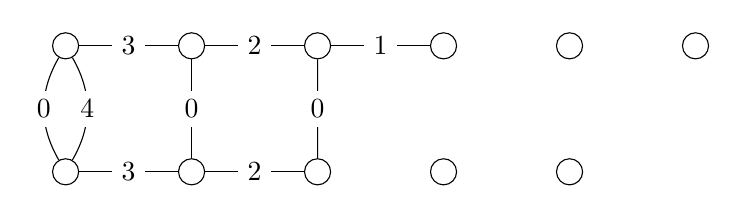
\begin{tikzpicture}[scale=.8]

        \begin{scope}[every node/.style={circle,draw}]
          \node (1)  at (0,2)  {};
          \node (2)  at (0,0)  {};
          \node (3)  at (2,2)  {};
          \node (4)  at (2,0)  {};
          \node (5)  at (4,2)  {};
          \node (6)  at (4,0)  {};
          \node (7)  at (6,2)  {};
          \node (8)  at (6,0)  {};
          \node (9)  at (8,2)  {};
          \node (10) at (8,0)  {};
          \node (11) at (10,2) {};
        \end{scope}

        \begin{scope}[every node/.style={fill=white}]

          \begin{scope}[every edge/.style={draw}]
            \path (1)  edge[bend right=30] node {$0$} (2);
            \path (3)  edge node {$0$} (4);
            \path (5)  edge node {$0$} (6);
            \path (5)  edge node {$1$} (7);
            \path (3)  edge node {$2$} (5);
            \path (4)  edge node {$2$} (6);
            \path (1)  edge node {$3$} (3);
            \path (2)  edge node {$3$} (4);
            \path (1)  edge[bend left=30] node {$4$} (2);
          \end{scope}
        \end{scope}

      \end{tikzpicture}
      \caption{Cas 1.1.2: doubles carrés alternés et arêtes doublées}
    \end{center}
  \end{figure}

  \paragraph{}
  We have two issues in this graphs: there is only one $\rho_4$ edge and if we link all remaining points with single edge, the total number of edges will be odd.

  \paragraph{}
  The $\rho_4$ edge cannot be place on the existing graph. So it must be placed between two fixed points. Then we need to link this edge to the rest of the graph, and because we have only two points, remaining, it must be done using a $\rho_2$ and $\rho_3$ edge. For now, we have the following graph:


  \begin{figure}[H]
    \begin{center}
      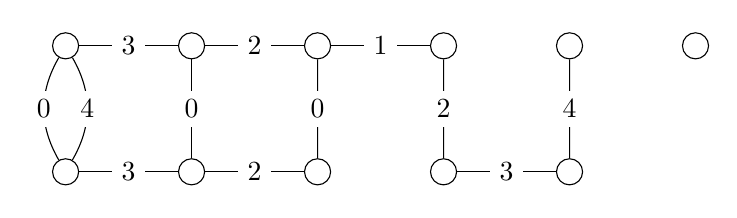
\begin{tikzpicture}[scale=.8]

        \begin{scope}[every node/.style={circle,draw}]
          \node (1)  at (0,2)  {};
          \node (2)  at (0,0)  {};
          \node (3)  at (2,2)  {};
          \node (4)  at (2,0)  {};
          \node (5)  at (4,2)  {};
          \node (6)  at (4,0)  {};
          \node (7)  at (6,2)  {};
          \node (8)  at (6,0)  {};
          \node (9)  at (8,2)  {};
          \node (10) at (8,0)  {};
          \node (11) at (10,2) {};
        \end{scope}

        \begin{scope}[every node/.style={fill=white}]

          \begin{scope}[every edge/.style={draw}]
            \path (1)  edge[bend right=30] node {$0$} (2);
            \path (3)  edge node {$0$} (4);
            \path (5)  edge node {$0$} (6);
            \path (5)  edge node {$1$} (7);
            \path (3)  edge node {$2$} (5);
            \path (4)  edge node {$2$} (6);
            \path (7)  edge node {$2$} (8);
            \path (1)  edge node {$3$} (3);
            \path (2)  edge node {$3$} (4);
            \path (8)  edge node {$3$} (10);
            \path (1)  edge[bend left=30] node {$4$} (2);
            \path (9)  edge node {$4$} (10);
          \end{scope}
        \end{scope}

      \end{tikzpicture}
      \caption{Cas 1.1.2: doubles carrés alternés et arêtes doublées}
    \end{center}
  \end{figure}

  \paragraph{}
  If wa want that the total number of point must be even, we must link the last point we a double edge. But that is impossile because the only point where we can start a double edge is the end of the $\rho_4$ edge but the the double edge must be $(\rho_3, \rho_5)$ but $\rho_5$ does not exists. Thus we cannot have a double edge between $\rho_0$ and $\rho_4$ in a permutation representation graph of $A_{11}$.


\end{proof}

\begin{corollary}
  \label{0-4-no-share}
  $\rho_0$ and $\rho_4$ edges cannot share a vertex.
\end{corollary}

\begin{proof}
  This can be directly deduced of Lemmas ~\ref{lemma-forbidden-alternating-square} and~\ref{lemma-forbidden-double-edge}.
\end{proof}

\section{Main theorems}

\begin{lemma}
  $\rho_0$ (and thus $\rho_4$) cannot be a 4-transposition.
\end{lemma}

\begin{proof}
  Suppose that $\rho_0$ is a 4-transposition

  \paragraph{}
  The $\rho_4$ involution must placed on the graph such that it commutes with $\rho_0$. The following patterns are possible for each $\rho_4$ edge:
  \begin{enumerate}
    \item Form an alternating square
    \item Double an existing edge
    \item Link two fixed points
  \end{enumerate}

  \paragraph{}
  The last pattern can only be used once because we only have three fixed points. But either $\rho_4$ is a 4-transposition or a 2-transposition, it is, at least, one edge that must still be placed. Thus, we must use one of the two other possibilities but then $\rho_0$ and $\rho_4$ will share a vertex which is impossible.
\end{proof}

We can now split our analysis in two cases dependending of the disposition of 4-tranpositions:
\begin{enumerate}
  \item $\rho_1$ is a 4-transpositions (whatever $\rho_3$ is)
  \item $\rho_1$ and $\rho_3$ are 2-transposition. If $\rho_3$ is a 4-transposition but $\rho_1$ not, we can take the dual and reduce it to the first case.
\end{enumerate}

\subsection{$\rho_1$ is a 4-transposition}

\paragraph{}
The objective of this section is to prove the following theorem in the two first cases:
\begin{theorem}
  If $\rho_1$ is a 4-transposition, then a generator can be written as a product of other generators, and thus the generating set is not free, so the group is not a sggi.
\end{theorem}

\paragraph{}
Let's draw a graph on which we place all edges of the 4-transposition $\rho_1$.

\begin{figure}[H]
  \begin{center}
    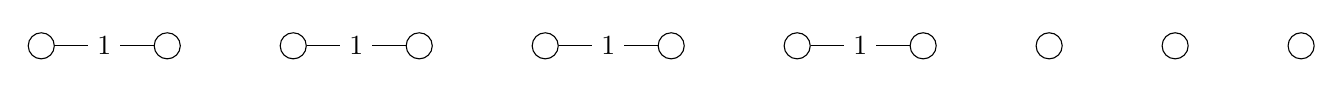
\begin{tikzpicture}[scale=.8]

      \begin{scope}[every node/.style={circle,draw}]
        \node (1)  at (0,0)  {};
        \node (2)  at (2,0)  {};
        \node (3)  at (4,0)  {};
        \node (4)  at (6,0)  {};
        \node (5)  at (8,0)  {};
        \node (6)  at (10,0)  {};
        \node (7)  at (12,0)  {};
        \node (8)  at (14,0)  {};
        \node (9)  at (16,0)  {};
        \node (10) at (18,0)  {};
        \node (11) at (20,0) {};
      \end{scope}

      \begin{scope}[every node/.style={fill=white}]

        \begin{scope}[every edge/.style={draw}]
          \path (1)  edge node {$1$} (2);
          \path (3)  edge node {$1$} (4);
          \path (5)  edge node {$1$} (6);
          \path (7)  edge node {$1$} (8);
        \end{scope}
      \end{scope}

    \end{tikzpicture}
    \caption{}
  \end{center}
\end{figure}

\paragraph{}
This transposition must commute with $\rho_3$ and $\rho_4$. We want to place the edge for $\rho_4$. They must commute with thoses of $\rho_1$, so for the two first edges, we have three possibilities: we can build an alternating square, double two edges or double one edge an link two fixed points.

\paragraph{}
Let's consider the first case, the alternating square:

\begin{figure}[H]
  \begin{center}
    \begin{tikzpicture}[scale=.8]

      \begin{scope}[every node/.style={circle,draw}]
        \node (1)  at (0,2)  {};
        \node (2)  at (0,0)  {};
        \node (3)  at (2,2)  {};
        \node (4)  at (2,0)  {};
        \node (5)  at (4,0)  {};
        \node (6)  at (6,0)  {};
        \node (7)  at (8,0)  {};
        \node (8)  at (10,0)  {};
        \node (9)  at (12,0)  {};
        \node (10) at (14,0)  {};
        \node (11) at (16,0) {};
      \end{scope}

      \begin{scope}[every node/.style={fill=white}]

        \begin{scope}[every edge/.style={draw}]
          \path (1)  edge node {$1$} (2);
          \path (3)  edge node {$1$} (4);
          \path (5)  edge node {$1$} (6);
          \path (7)  edge node {$1$} (8);
          \path (1)  edge node {$4$} (3);
          \path (2)  edge node {$4$} (4);
        \end{scope}
      \end{scope}

    \end{tikzpicture}
    \caption{}
  \end{center}
\end{figure}

\paragraph{}
If $\rho_4$ forms an alternating square with $\rho_1$, it must be adjacent to an other alternating square between $\rho_1$ and $\rho_3$ ($\rho_2$ and $\rho_4$ is not possible because $\rho_4$ is a 2-transposition). The sequence of square cannot be extended in this direction because we will need to build 2 extra alternating square and we cannot place a rotation pattern and so we would need 2 extra $\rho_1$ edge but there is only one.

\paragraph{}
If it's extended in the other direction, we would use the last $\rho_1$ edge and two $\rho_3$ edge. At the end, there will remain only 2 $\rho_0$ edges and 2 or 4 $\rho_2$ edges. But the cannot form a connex graph. We will remain with our 2 alternating squares. Thoses squares must be linked to the rest of the graph by a $\rho_2$ edge. But there are still 2 $\rho_0$ edge to place.

\begin{figure}[H]
  \begin{center}
    \begin{tikzpicture}[scale=.8]

      \begin{scope}[every node/.style={circle,draw}]
        \node (1)  at (0,2)  {};
        \node (2)  at (0,0)  {};
        \node (3)  at (2,2)  {};
        \node (4)  at (2,0)  {};
        \node (5)  at (4,2)  {};
        \node (6)  at (4,0)  {};
        \node (7)  at (6,0)  {};
        \node (8)  at (8,0)  {};
        \node (9)  at (10,0)  {};
        \node (10) at (12,0)  {};
        \node (11) at (14,0) {};
      \end{scope}

      \begin{scope}[every node/.style={fill=white}]

        \begin{scope}[every edge/.style={draw}]
          \path (1)  edge node {$1$} (2);
          \path (3)  edge node {$1$} (4);
          \path (5)  edge node {$1$} (6);
          \path (7)  edge node {$1$} (8);
          \path (3)  edge node {$3$} (5);
          \path (4)  edge node {$3$} (6);
          \path (1)  edge node {$4$} (3);
          \path (2)  edge node {$4$} (4);
        \end{scope}
      \end{scope}

    \end{tikzpicture}
    \caption{}
  \end{center}
\end{figure}


\paragraph{}
Now let's place the two $\rho_0$ edges. They must touch at least one $\rho_1$ edge, otherwise $\rho_0$ and $\rho_1$ would commute but that's impossible.

\paragraph{}
Recall that, by Lemmas~\ref{lemma-forbidden-alternating-square} and~\ref{lemma-forbidden-double-edge}, we know that the edges of involutions $\rho_0$ and $\rho_4$ cannot share a vertex. So the $\rho_0$ edge cannot be linked to the first 4 vertices. They cannot be connected thus to the 5th and 6th vertices because it would form an alternating square but we choose to not make one at this position. The cannot be connected to the end of the $\rho_2$ too.

\paragraph{}
The only remaining possibility is to link the extremity of the compoenent with a single $\rho_1$ edge to a fixed point. The other $\rho_0$ edge must link the two fixed points because if we used to other extremity of the single $\rho_1$ edge, we would not be able to connect it to anything because all $\rho_1$ would have been already used.

\begin{figure}[H]
  \begin{center}
    \begin{tikzpicture}[scale=.8]

      \begin{scope}[every node/.style={circle,draw}]
        \node (1)  at (0,2)  {};
        \node (2)  at (0,0)  {};
        \node (3)  at (2,2)  {};
        \node (4)  at (2,0)  {};
        \node (5)  at (4,2)  {};
        \node (6)  at (4,0)  {};
        \node (7)  at (6,0)  {};
        \node (8)  at (8,0)  {};
        \node (9)  at (10,0)  {};
        \node (10) at (12,0)  {};
        \node (11) at (14,0) {};
      \end{scope}

      \begin{scope}[every node/.style={fill=white}]

        \begin{scope}[every edge/.style={draw}]
          \path (8)  edge node {$0$} (9);
          \path (10)  edge node {$0$} (11);
          \path (1)  edge node {$1$} (2);
          \path (3)  edge node {$1$} (4);
          \path (5)  edge node {$1$} (6);
          \path (7)  edge node {$1$} (8);
          \path (3)  edge node {$3$} (5);
          \path (4)  edge node {$3$} (6);
          \path (1)  edge node {$4$} (3);
          \path (2)  edge node {$4$} (4);
        \end{scope}
      \end{scope}

    \end{tikzpicture}
    \caption{}
  \end{center}
\end{figure}

\paragraph{}
The two alternating square can only be linked by a $\rho_2$ edge. This edge must be linked to the $\rho_1$ component because we choosed to not make an alternating square at this place.

\begin{figure}[H]
  \begin{center}
    \begin{tikzpicture}[scale=.8]

      \begin{scope}[every node/.style={circle,draw}]
        \node (1)  at (0,2)  {};
        \node (2)  at (0,0)  {};
        \node (3)  at (2,2)  {};
        \node (4)  at (2,0)  {};
        \node (5)  at (4,2)  {};
        \node (6)  at (4,0)  {};
        \node (7)  at (6,0)  {};
        \node (8)  at (8,0)  {};
        \node (9)  at (10,0)  {};
        \node (10) at (12,0)  {};
        \node (11) at (14,0) {};
      \end{scope}

      \begin{scope}[every node/.style={fill=white}]

        \begin{scope}[every edge/.style={draw}]
          \path (8)  edge node {$0$} (9);
          \path (10)  edge node {$0$} (11);
          \path (1)  edge node {$1$} (2);
          \path (3)  edge node {$1$} (4);
          \path (5)  edge node {$1$} (6);
          \path (7)  edge node {$1$} (8);
          \path (6)  edge node {$2$} (7);
          \path (3)  edge node {$3$} (5);
          \path (4)  edge node {$3$} (6);
          \path (1)  edge node {$4$} (3);
          \path (2)  edge node {$4$} (4);
        \end{scope}
      \end{scope}

    \end{tikzpicture}
    \caption{}
  \end{center}
\end{figure}

\paragraph{}
All $\rho_1$ edges have been used, they cannot be used to link the single $\rho_0$. Therefore we must used an alternating square to connect it. But this alternating square must be connected directly. Therefore the difference between the indices of the edges must be 2. The vertical edges of the square must therefore be $\rho_2$.

\begin{figure}[H]
  \begin{center}
    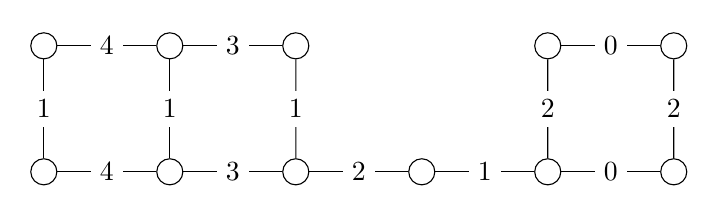
\begin{tikzpicture}[scale=.8]

      \begin{scope}[every node/.style={circle,draw}]
        \node (1)  at (0,2)  {};
        \node (2)  at (0,0)  {};
        \node (3)  at (2,2)  {};
        \node (4)  at (2,0)  {};
        \node (5)  at (4,2)  {};
        \node (6)  at (4,0)  {};
        \node (7)  at (6,0)  {};
        \node (8)  at (8,2)  {};
        \node (9)  at (8,0)  {};
        \node (10) at (10,2)  {};
        \node (11) at (10,0) {};
      \end{scope}

      \begin{scope}[every node/.style={fill=white}]

        \begin{scope}[every edge/.style={draw}]
          \path (9)  edge node {$0$} (11);
          \path (8)  edge node {$0$} (10);
          \path (1)  edge node {$1$} (2);
          \path (3)  edge node {$1$} (4);
          \path (5)  edge node {$1$} (6);
          \path (7)  edge node {$1$} (9);
          \path (6)  edge node {$2$} (7);
          \path (8)  edge node {$2$} (9);
          \path (10) edge node {$2$} (11);
          \path (3)  edge node {$3$} (5);
          \path (4)  edge node {$3$} (6);
          \path (1)  edge node {$4$} (3);
          \path (2)  edge node {$4$} (4);
        \end{scope}
      \end{scope}

    \end{tikzpicture}
    \caption{Un carré alterné et son voisin engendré}
  \end{center}
\end{figure}

\paragraph{}
There are only 3 $\rho_2$ edges on this graph. A last one must be added to restore parity. There is only two places possible:  we can double any of the $\rho_4$ edge. That gives us 2 graphs:

\begin{figure}[H]
  \begin{center}
    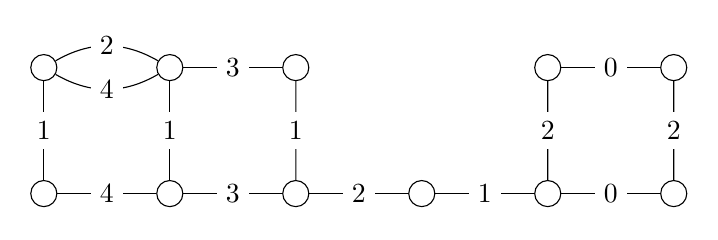
\begin{tikzpicture}[scale=.8]

      \begin{scope}[every node/.style={circle,draw}]
        \node (1)  at (0,2)  {};
        \node (2)  at (0,0)  {};
        \node (3)  at (2,2)  {};
        \node (4)  at (2,0)  {};
        \node (5)  at (4,2)  {};
        \node (6)  at (4,0)  {};
        \node (7)  at (6,0)  {};
        \node (8)  at (8,2)  {};
        \node (9)  at (8,0)  {};
        \node (10) at (10,2)  {};
        \node (11) at (10,0) {};
      \end{scope}

      \begin{scope}[every node/.style={fill=white}]

        \begin{scope}[every edge/.style={draw}]
          \path (9)  edge node {$0$} (11);
          \path (8)  edge node {$0$} (10);
          \path (1)  edge node {$1$} (2);
          \path (3)  edge node {$1$} (4);
          \path (5)  edge node {$1$} (6);
          \path (7)  edge node {$1$} (9);
          \path (1)  edge[bend left=30] node {$2$} (3);
          \path (6)  edge node {$2$} (7);
          \path (8)  edge node {$2$} (9);
          \path (10) edge node {$2$} (11);
          \path (3)  edge node {$3$} (5);
          \path (4)  edge node {$3$} (6);
          \path (1)  edge[bend right=30] node {$4$} (3);
          \path (2)  edge node {$4$} (4);
        \end{scope}
      \end{scope}

    \end{tikzpicture}
    \caption{Un carré alterné et son voisin engendré}
  \end{center}
\end{figure}

\begin{figure}[H]
  \begin{center}
    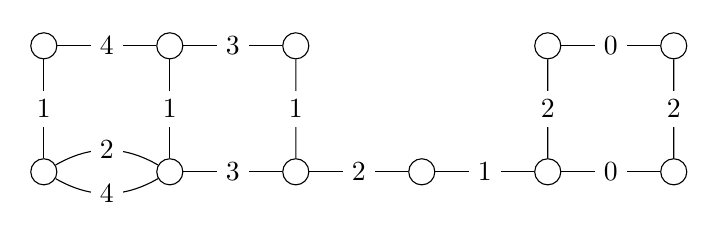
\begin{tikzpicture}[scale=.8]

      \begin{scope}[every node/.style={circle,draw}]
        \node (1)  at (0,2)  {};
        \node (2)  at (0,0)  {};
        \node (3)  at (2,2)  {};
        \node (4)  at (2,0)  {};
        \node (5)  at (4,2)  {};
        \node (6)  at (4,0)  {};
        \node (7)  at (6,0)  {};
        \node (8)  at (8,2)  {};
        \node (9)  at (8,0)  {};
        \node (10) at (10,2)  {};
        \node (11) at (10,0) {};
      \end{scope}

      \begin{scope}[every node/.style={fill=white}]

        \begin{scope}[every edge/.style={draw}]
          \path (9)  edge node {$0$} (11);
          \path (8)  edge node {$0$} (10);
          \path (1)  edge node {$1$} (2);
          \path (3)  edge node {$1$} (4);
          \path (5)  edge node {$1$} (6);
          \path (7)  edge node {$1$} (9);
          \path (2)  edge[bend left=30] node {$2$} (4);
          \path (6)  edge node {$2$} (7);
          \path (8)  edge node {$2$} (9);
          \path (10) edge node {$2$} (11);
          \path (3)  edge node {$3$} (5);
          \path (4)  edge node {$3$} (6);
          \path (1)  edge node {$4$} (3);
          \path (2)  edge[bend right=30] node {$4$} (4);
        \end{scope}
      \end{scope}

    \end{tikzpicture}
    \caption{Un carré alterné et son voisin engendré}
  \end{center}
\end{figure}

\paragraph{}
But $\rho_3$ is currently a 2-transposition, we can stop here or try to convert $\rho_3$ to a 4-transposition. If we look where we can place an extra $\rho_3$ edge, there are two positions for two edges: double the left $\rho_1$ edge and double the right $\rho_0$ edge. That creates two other graphs:

\begin{figure}[H]
  \begin{center}
    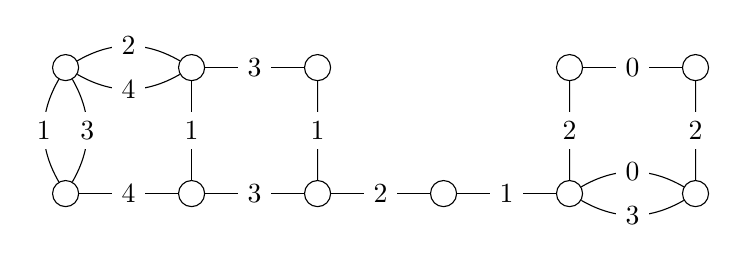
\begin{tikzpicture}[scale=.8]

      \begin{scope}[every node/.style={circle,draw}]
        \node (1)  at (0,2)  {};
        \node (2)  at (0,0)  {};
        \node (3)  at (2,2)  {};
        \node (4)  at (2,0)  {};
        \node (5)  at (4,2)  {};
        \node (6)  at (4,0)  {};
        \node (7)  at (6,0)  {};
        \node (8)  at (8,2)  {};
        \node (9)  at (8,0)  {};
        \node (10) at (10,2)  {};
        \node (11) at (10,0) {};
      \end{scope}

      \begin{scope}[every node/.style={fill=white}]

        \begin{scope}[every edge/.style={draw}]
          \path (9)  edge[bend left=30] node {$0$} (11);
          \path (8)  edge node {$0$} (10);
          \path (1)  edge[bend right=30] node {$1$} (2);
          \path (3)  edge node {$1$} (4);
          \path (5)  edge node {$1$} (6);
          \path (7)  edge node {$1$} (9);
          \path (1)  edge[bend left=30] node {$2$} (3);
          \path (6)  edge node {$2$} (7);
          \path (8)  edge node {$2$} (9);
          \path (10) edge node {$2$} (11);
          \path (1)  edge[bend left=30] node {$3$} (2);
          \path (3)  edge node {$3$} (5);
          \path (4)  edge node {$3$} (6);
          \path (9)  edge[bend right=30] node {$3$} (11);
          \path (1)  edge[bend right=30] node {$4$} (3);
          \path (2)  edge node {$4$} (4);
        \end{scope}
      \end{scope}

    \end{tikzpicture}
    \caption{Un carré alterné et son voisin engendré}
  \end{center}
\end{figure}

\begin{figure}[H]
  \begin{center}
    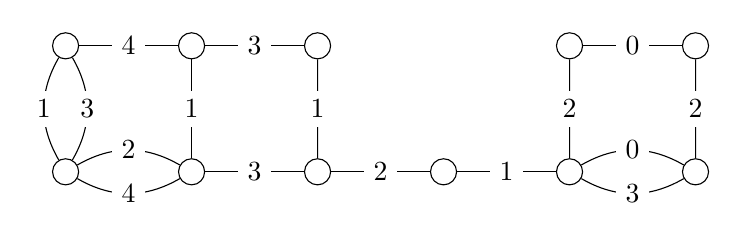
\begin{tikzpicture}[scale=.8]

      \begin{scope}[every node/.style={circle,draw}]
        \node (1)  at (0,2)  {};
        \node (2)  at (0,0)  {};
        \node (3)  at (2,2)  {};
        \node (4)  at (2,0)  {};
        \node (5)  at (4,2)  {};
        \node (6)  at (4,0)  {};
        \node (7)  at (6,0)  {};
        \node (8)  at (8,2)  {};
        \node (9)  at (8,0)  {};
        \node (10) at (10,2)  {};
        \node (11) at (10,0) {};
      \end{scope}

      \begin{scope}[every node/.style={fill=white}]

        \begin{scope}[every edge/.style={draw}]
          \path (9)  edge[bend left=30] node {$0$} (11);
          \path (8)  edge node {$0$} (10);
          \path (1)  edge[bend right=30] node {$1$} (2);
          \path (3)  edge node {$1$} (4);
          \path (5)  edge node {$1$} (6);
          \path (7)  edge node {$1$} (9);
          \path (2)  edge[bend left=30] node {$2$} (4);
          \path (6)  edge node {$2$} (7);
          \path (8)  edge node {$2$} (9);
          \path (10) edge node {$2$} (11);
          \path (1)  edge[bend left=30] node {$3$} (2);
          \path (3)  edge node {$3$} (5);
          \path (4)  edge node {$3$} (6);
          \path (9)  edge[bend right=30] node {$3$} (11);
          \path (1)  edge node {$4$} (3);
          \path (2)  edge[bend right=30] node {$4$} (4);
        \end{scope}
      \end{scope}

    \end{tikzpicture}
    \caption{Un carré alterné et son voisin engendré}
  \end{center}
\end{figure}

\paragraph{}
Let's go back to the case where $\rho_3$ is a 2-transposition. Let's remove all edges from involutions $\rho_0$ and $\rho_3$, We have the following graph.

\begin{figure}[H]
  \begin{center}
    \begin{tikzpicture}[scale=.8]

      \begin{scope}[every node/.style={circle,draw}]
        \node (1)  at (0,2)  {};
        \node (2)  at (0,0)  {};
        \node (3)  at (2,2)  {};
        \node (4)  at (2,0)  {};
        \node (5)  at (6,0)  {};
        \node (6)  at (4,0)  {};
        \node (7)  at (8,0)  {};
        \node (8)  at (10,0)  {};
        \node (9)  at (12,0)  {};
        \node (10) at (14,0)  {};
        \node (11) at (16,0) {};
      \end{scope}

      \begin{scope}[every node/.style={fill=white}]

        \begin{scope}[every edge/.style={draw}]
          \path (1)  edge node {$1$} (2);
          \path (3)  edge node {$1$} (4);
          \path (5)  edge node {$1$} (6);
          \path (7)  edge node {$1$} (8);
          \path (1)  edge[bend left=30] node {$2$} (3);
          \path (5)  edge node {$2$} (7);
          \path (8)  edge node {$2$} (9);
          \path (10) edge node {$2$} (11);
          \path (1)  edge[bend right=30] node {$4$} (3);
          \path (2)  edge node {$4$} (4);
        \end{scope}
      \end{scope}

    \end{tikzpicture}
    \caption{Un carré alterné et son voisin engendré}
  \end{center}
\end{figure}

\paragraph{}
Now we can see easily that $\rho_4 = (\rho_1 \rho_2)^{10}$. The set of generators is not free and so it's not a generating set.

\paragraph{}
When $\rho_3$ is a 4-transposition, the same applies.

\paragraph{}
This conclude our analysis for the alternating square between $\rho_1$ and $\rho_4$. The second possibility is having a double edge with involutions $\rho_0$ and $\rho_4$. We must place an alternating square next to it because this double must be connected to the rest of the graph. We have two possibilities for the alternating square: $[\rho_1, \rho_3]$ or $[\rho_2, \rho_4]$. In the first case, we have the following graph:

\begin{figure}[H]
  \begin{center}
    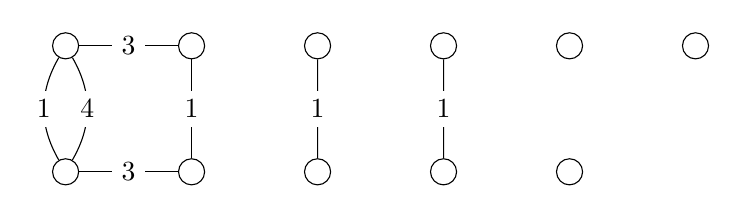
\begin{tikzpicture}[scale=.8]

      \begin{scope}[every node/.style={circle,draw}]
        \node (1)  at (0,2)  {};
        \node (2)  at (0,0)  {};
        \node (3)  at (2,2)  {};
        \node (4)  at (2,0)  {};
        \node (5)  at (4,2)  {};
        \node (6)  at (4,0)  {};
        \node (7)  at (6,2)  {};
        \node (8)  at (6,0)  {};
        \node (9)  at (8,2)  {};
        \node (10) at (8,0)  {};
        \node (11) at (10,2) {};
      \end{scope}

      \begin{scope}[every node/.style={fill=white}]

        \begin{scope}[every edge/.style={draw}]
          \path (1)  edge[bend right=30] node {$1$} (2);
          \path (3)  edge node {$1$} (4);
          \path (5)  edge node {$1$} (6);
          \path (7)  edge node {$1$} (8);
          \path (1)  edge node {$3$} (3);
          \path (2)  edge node {$3$} (4);
          \path (1)  edge[bend left=30] node {$4$} (2);
        \end{scope}
      \end{scope}

    \end{tikzpicture}
    \caption{Un carré alterné et son voisin engendré}
  \end{center}
\end{figure}

\paragraph{}
Recall that $\rho_0$ and $\rho_1$ must not commute. Therefore a $\rho_0$ edge must be connected to at least one $\rho_1$ edge. Therefore at least one $\rho_1$ edge must not be part of an alternating square that does not also use $\rho_0$.

\paragraph{}
This alternating square cannot be linked by another alternating square on the right because it will need two alternating square on the right of we are not changing the value of the vertical edges. But that will place all $\rho_1$ in alternating squares. We must therefore change the value of the vertical edges. But the horizontal edges of the second square must be $\rho_2$ because there if not enough $\rho_4$ edge. But then the new value for vertical edge must be adjacent to $\rho_3$. $\rho_2$ is impossible because it is already used for the horizontal edges. The only remaining possibility is $\rho_4$ but if we want to build an alternating square, we will need 2 $\rho_4$ but there are only 2 in total and one has already been used.

\paragraph{}
If we attach an alternating square on the left, it must be a $[\rho_2, \rho_4]$ alternating square. The graph is the following:

\begin{figure}[H]
  \begin{center}
    \begin{tikzpicture}[scale=.8]

      \begin{scope}[every node/.style={circle,draw}]
        \node (1)  at (0,2)  {};
        \node (2)  at (0,0)  {};
        \node (3)  at (2,2)  {};
        \node (4)  at (2,0)  {};
        \node (5)  at (4,0)  {};
        \node (6)  at (6,0)  {};
        \node (7)  at (8,0)  {};
        \node (8)  at (10,0)  {};
        \node (9)  at (-2,2)  {};
        \node (10) at (-2,0)  {};
        \node (11) at (12,0) {};
      \end{scope}

      \begin{scope}[every node/.style={fill=white}]

        \begin{scope}[every edge/.style={draw}]
          \path (1)  edge[bend right=30] node {$1$} (2);
          \path (3)  edge node {$1$} (4);
          \path (5)  edge node {$1$} (6);
          \path (7)  edge node {$1$} (8);
          \path (1)  edge node {$2$} (9);
          \path (2)  edge node {$2$} (10);
          \path (1)  edge node {$3$} (3);
          \path (2)  edge node {$3$} (4);
          \path (1)  edge[bend left=30] node {$4$} (2);
          \path (9)  edge node {$4$} (10);
        \end{scope}
      \end{scope}

    \end{tikzpicture}
    \caption{Un carré alterné et son voisin engendré}
  \end{center}
\end{figure}

\paragraph{}
Now we must place the two $\rho_0$ edges, they cannot be placed on any vertex of the left component. They must therefore link the $\rho_1$ edges and the fixed points. The fixed point can only be linked once and each $\rho_1$ edge can be linked twice. But we cannot link the $\rho_1$ edges together twice because it will just form an alternating square and then the involutions commutes. The only remaining possibility is to link the fixed point to a $\rho_1$ edge and the two $\rho_1$ edges together.

\begin{figure}[H]
  \begin{center}
    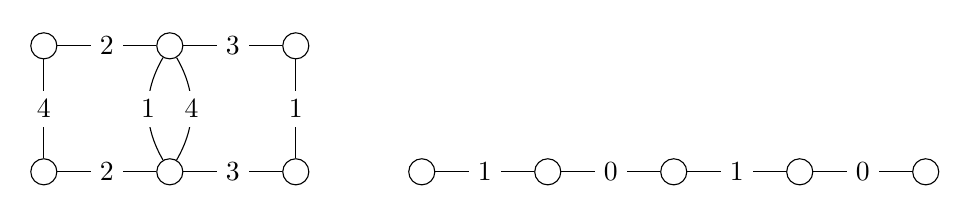
\begin{tikzpicture}[scale=.8]

      \begin{scope}[every node/.style={circle,draw}]
        \node (1)  at (0,2)  {};
        \node (2)  at (0,0)  {};
        \node (3)  at (2,2)  {};
        \node (4)  at (2,0)  {};
        \node (5)  at (4,0)  {};
        \node (6)  at (6,0)  {};
        \node (7)  at (8,0)  {};
        \node (8)  at (10,0)  {};
        \node (9)  at (-2,2)  {};
        \node (10) at (-2,0)  {};
        \node (11) at (12,0) {};
      \end{scope}

      \begin{scope}[every node/.style={fill=white}]

        \begin{scope}[every edge/.style={draw}]
          \path (6)  edge node {$0$} (7);
          \path (8)  edge node {$0$} (11);
          \path (1)  edge[bend right=30] node {$1$} (2);
          \path (3)  edge node {$1$} (4);
          \path (5)  edge node {$1$} (6);
          \path (7)  edge node {$1$} (8);
          \path (1)  edge node {$2$} (9);
          \path (2)  edge node {$2$} (10);
          \path (1)  edge node {$3$} (3);
          \path (2)  edge node {$3$} (4);
          \path (1)  edge[bend left=30] node {$4$} (2);
          \path (9)  edge node {$4$} (10);
        \end{scope}
      \end{scope}

    \end{tikzpicture}
    \caption{Un carré alterné et son voisin engendré}
  \end{center}
\end{figure}

\paragraph{}
Now the two components must be linked by a $\rho_2$ edge but the total number of $\rho_2$ edges becomes odd. Another $\rho_2$ must be placed but the only possibilites are to double a $\rho_0$ edge. Therefore, we have two possible graphs.

\begin{figure}[H]
  \begin{center}
    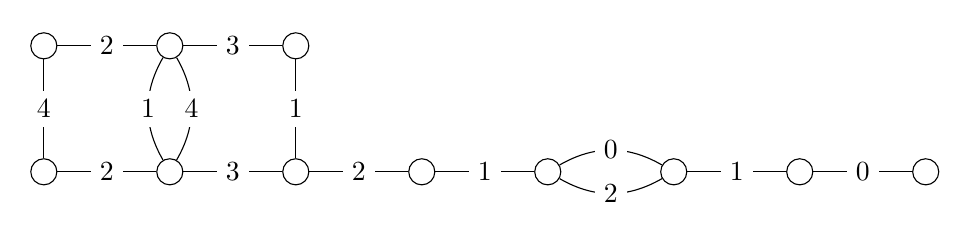
\begin{tikzpicture}[scale=.8]

      \begin{scope}[every node/.style={circle,draw}]
        \node (1)  at (0,2)  {};
        \node (2)  at (0,0)  {};
        \node (3)  at (2,2)  {};
        \node (4)  at (2,0)  {};
        \node (5)  at (4,0)  {};
        \node (6)  at (6,0)  {};
        \node (7)  at (8,0)  {};
        \node (8)  at (10,0)  {};
        \node (9)  at (-2,2)  {};
        \node (10) at (-2,0)  {};
        \node (11) at (12,0) {};
      \end{scope}

      \begin{scope}[every node/.style={fill=white}]

        \begin{scope}[every edge/.style={draw}]
          \path (6)  edge[bend left=30] node {$0$} (7);
          \path (8)  edge node {$0$} (11);
          \path (1)  edge[bend right=30] node {$1$} (2);
          \path (3)  edge node {$1$} (4);
          \path (5)  edge node {$1$} (6);
          \path (7)  edge node {$1$} (8);
          \path (1)  edge node {$2$} (9);
          \path (2)  edge node {$2$} (10);
          \path (4)  edge node {$2$} (5);
          \path (6)  edge[bend right=30] node {$2$} (7);
          \path (1)  edge node {$3$} (3);
          \path (2)  edge node {$3$} (4);
          \path (1)  edge[bend left=30] node {$4$} (2);
          \path (9)  edge node {$4$} (10);
        \end{scope}
      \end{scope}

    \end{tikzpicture}
    \caption{Un carré alterné et son voisin engendré}
  \end{center}
\end{figure}

\begin{figure}[H]
  \begin{center}
    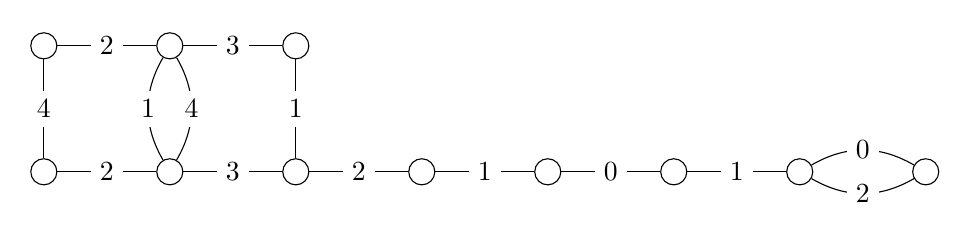
\begin{tikzpicture}[scale=.8]

      \begin{scope}[every node/.style={circle,draw}]
        \node (1)  at (0,2)  {};
        \node (2)  at (0,0)  {};
        \node (3)  at (2,2)  {};
        \node (4)  at (2,0)  {};
        \node (5)  at (4,0)  {};
        \node (6)  at (6,0)  {};
        \node (7)  at (8,0)  {};
        \node (8)  at (10,0)  {};
        \node (9)  at (-2,2)  {};
        \node (10) at (-2,0)  {};
        \node (11) at (12,0) {};
      \end{scope}

      \begin{scope}[every node/.style={fill=white}]

        \begin{scope}[every edge/.style={draw}]
          \path (6)  edge node {$0$} (7);
          \path (8)  edge[bend left=30] node {$0$} (11);
          \path (1)  edge[bend right=30] node {$1$} (2);
          \path (3)  edge node {$1$} (4);
          \path (5)  edge node {$1$} (6);
          \path (7)  edge node {$1$} (8);
          \path (1)  edge node {$2$} (9);
          \path (2)  edge node {$2$} (10);
          \path (4)  edge node {$2$} (5);
          \path (8)  edge[bend right=30] node {$2$} (11);
          \path (1)  edge node {$3$} (3);
          \path (2)  edge node {$3$} (4);
          \path (1)  edge[bend left=30] node {$4$} (2);
          \path (9)  edge node {$4$} (10);
        \end{scope}
      \end{scope}

    \end{tikzpicture}
    \caption{Un carré alterné et son voisin engendré}
  \end{center}
\end{figure}

\paragraph{}
In those graph, if the $\rho_4$ edge is removed, the generated group remains 2-transitive\footnote{TODO} and thus primitive. By looking at the size of the subgroups, it is possible to deduce that the generated group

\paragraph{}
Now let's look at the case when we start with a $[\rho_2,  \rho_4]$ square.

\begin{figure}[H]
  \begin{center}
    \begin{tikzpicture}[scale=.8]

      \begin{scope}[every node/.style={circle,draw}]
        \node (1)  at (0,2)  {};
        \node (2)  at (0,0)  {};
        \node (3)  at (2,2)  {};
        \node (4)  at (2,0)  {};
        \node (5)  at (6,0)  {};
        \node (6)  at (4,0)  {};
        \node (7)  at (10,0)  {};
        \node (8)  at (8,0)  {};
        \node (9)  at (12,0)  {};
        \node (10) at (14,0)  {};
        \node (11) at (16,0) {};
      \end{scope}

      \begin{scope}[every node/.style={fill=white}]

        \begin{scope}[every edge/.style={draw}]
          \path (1)  edge[bend right=30] node {$1$} (2);
          \path (5)  edge node {$1$} (6);
          \path (7)  edge node {$1$} (8);
          \path (9)  edge node {$1$} (10);
          \path (1)  edge node {$2$} (3);
          \path (2)  edge node {$2$} (4);
          \path (1)  edge[bend left=30] node {$4$} (2);
          \path (3)  edge node {$4$} (4);
        \end{scope}
      \end{scope}

    \end{tikzpicture}
    \caption{Un carré alterné et son voisin engendré}
  \end{center}
\end{figure}

\paragraph{}
Now you can add two extra alternating square or link this alternating square to some other component. But it's impossible to add another alternating square to right of this sequence because the vertical component cannot be another $\rho_4$ edge because we have used all. So we need to double right edge of the square but the only possibilites are $\rho_1$ and $\rho_3$ but $\rho_1$ is excluded by our previous choice. Therefore the vertical edge of the square must be double bu a $\rho_3$ edge but the horizontal component of the new sqaure must also be $\rho_3$ but that is impossible.

\paragraph{}
The alternating square can however be extended to the left by a $[\rho_1, \rho_3]$ edge but then we can reduce it to the first case where we choose to build a $[\rho_1, \rho_3]$ square directly.

\paragraph{}
The only remaining possibility is to link to square to the rest of the graph with a single edge. We must use a $\rho_3$ edge. But we cannot connect to a $\rho_1$ edge because we will need to build an alterating square but we proved that is impossible. The only possibility is to link it to the fixed point. We have the following graph.

\begin{figure}[H]
  \begin{center}
    \begin{tikzpicture}[scale=.8]

      \begin{scope}[every node/.style={circle,draw}]
        \node (1)  at (0,2)  {};
        \node (2)  at (0,0)  {};
        \node (3)  at (2,2)  {};
        \node (4)  at (2,0)  {};
        \node (5)  at (8,0)  {};
        \node (6)  at (6,0)  {};
        \node (7)  at (12,0)  {};
        \node (8)  at (10,0)  {};
        \node (9)  at (14,0)  {};
        \node (10) at (16,0)  {};
        \node (11) at (4,0) {};
      \end{scope}

      \begin{scope}[every node/.style={fill=white}]

        \begin{scope}[every edge/.style={draw}]
          \path (1)  edge[bend right=30] node {$1$} (2);
          \path (5)  edge node {$1$} (6);
          \path (7)  edge node {$1$} (8);
          \path (9)  edge node {$1$} (10);
          \path (1)  edge node {$2$} (3);
          \path (2)  edge node {$2$} (4);
          \path (4)  edge node {$3$} (11);
          \path (1)  edge[bend left=30] node {$4$} (2);
          \path (3)  edge node {$4$} (4);
        \end{scope}
      \end{scope}

    \end{tikzpicture}
    \caption{Un carré alterné et son voisin engendré}
  \end{center}
\end{figure}

\paragraph{}
We still need to place two $\rho_0$ edges, they must not commute with $\rho_1$, thus at least one edge must link two $\rho_1$ involutions. But the other $\rho_0$ must link the two other $\rho_1$ edges.

\begin{figure}[H]
  \begin{center}
    \begin{tikzpicture}[scale=.8]

      \begin{scope}[every node/.style={circle,draw}]
        \node (1)  at (0,2)  {};
        \node (2)  at (0,0)  {};
        \node (3)  at (2,2)  {};
        \node (4)  at (2,0)  {};
        \node (5)  at (8,0)  {};
        \node (6)  at (6,0)  {};
        \node (7)  at (12,0)  {};
        \node (8)  at (10,0)  {};
        \node (9)  at (14,0)  {};
        \node (10) at (16,0)  {};
        \node (11) at (4,0) {};
      \end{scope}

      \begin{scope}[every node/.style={fill=white}]

        \begin{scope}[every edge/.style={draw}]
          \path (5)  edge node {$0$} (8);
          \path (7)  edge node {$0$} (9);
          \path (1)  edge[bend right=30] node {$1$} (2);
          \path (5)  edge node {$1$} (6);
          \path (7)  edge node {$1$} (8);
          \path (9)  edge node {$1$} (10);
          \path (1)  edge node {$2$} (3);
          \path (2)  edge node {$2$} (4);
          \path (4)  edge node {$3$} (11);
          \path (1)  edge[bend left=30] node {$4$} (2);
          \path (3)  edge node {$4$} (4);
        \end{scope}
      \end{scope}

    \end{tikzpicture}
    \caption{Un carré alterné et son voisin engendré}
  \end{center}
\end{figure}

\paragraph{}
We need to connect this point to the rest of the graph. But, since all $\rho_4$ edge have been used and since nothing can be connected to the alternating square, we must connect this point to a $\rho_1$ edge by a $\rho_2$ edge.

\begin{figure}[H]
  \begin{center}
    \begin{tikzpicture}[scale=.8]

      \begin{scope}[every node/.style={circle,draw}]
        \node (1)  at (0,2)  {};
        \node (2)  at (0,0)  {};
        \node (3)  at (2,2)  {};
        \node (4)  at (2,0)  {};
        \node (5)  at (8,0)  {};
        \node (6)  at (6,0)  {};
        \node (7)  at (12,0)  {};
        \node (8)  at (10,0)  {};
        \node (9)  at (14,0)  {};
        \node (10) at (16,0)  {};
        \node (11) at (4,0) {};
      \end{scope}

      \begin{scope}[every node/.style={fill=white}]

        \begin{scope}[every edge/.style={draw}]
          \path (5)  edge node {$0$} (8);
          \path (7)  edge node {$0$} (9);
          \path (1)  edge[bend right=30] node {$1$} (2);
          \path (5)  edge node {$1$} (6);
          \path (7)  edge node {$1$} (8);
          \path (9)  edge node {$1$} (10);
          \path (1)  edge node {$2$} (3);
          \path (2)  edge node {$2$} (4);
          \path (11)  edge node {$2$} (6);
          \path (4)  edge node {$3$} (11);
          \path (1)  edge[bend left=30] node {$4$} (2);
          \path (3)  edge node {$4$} (4);
        \end{scope}
      \end{scope}

    \end{tikzpicture}
    \caption{Un carré alterné et son voisin engendré}
  \end{center}
\end{figure}

\paragraph{}
Now we need to place a $\rho_3$ edge, the only possibility is to place it on the double edge. The $\rho_2$ edge must then be placed such that it double a $\rho_0$ edge. We have two graphs:


\begin{figure}[H]
  \begin{center}
    \begin{tikzpicture}[scale=.8]

      \begin{scope}[every node/.style={circle,draw}]
        \node (1)  at (0,2)  {};
        \node (2)  at (0,0)  {};
        \node (3)  at (2,2)  {};
        \node (4)  at (2,0)  {};
        \node (5)  at (8,0)  {};
        \node (6)  at (6,0)  {};
        \node (7)  at (12,0)  {};
        \node (8)  at (10,0)  {};
        \node (9)  at (14,0)  {};
        \node (10) at (16,0)  {};
        \node (11) at (4,0) {};
      \end{scope}

      \begin{scope}[every node/.style={fill=white}]

        \begin{scope}[every edge/.style={draw}]
          \path (5)  edge[bend left=30] node {$0$} (8);
          \path (7)  edge node {$0$} (9);
          \path (1)  edge[bend right=40] node {$1$} (2);
          \path (5)  edge node {$1$} (6);
          \path (7)  edge node {$1$} (8);
          \path (9)  edge node {$1$} (10);
          \path (1)  edge node {$2$} (3);
          \path (2)  edge node {$2$} (4);
          \path (5)  edge[bend right=30] node {$2$} (8);
          \path (11) edge node {$2$} (6);
          \path (1)  edge node {$3$} (2);
          \path (4)  edge node {$3$} (11);
          \path (1)  edge[bend left=40] node {$4$} (2);
          \path (3)  edge node {$4$} (4);
        \end{scope}
      \end{scope}

    \end{tikzpicture}
    \caption{Un carré alterné et son voisin engendré}
  \end{center}
\end{figure}

\begin{figure}[H]
  \begin{center}
    \begin{tikzpicture}[scale=.8]

      \begin{scope}[every node/.style={circle,draw}]
        \node (1)  at (0,2)  {};
        \node (2)  at (0,0)  {};
        \node (3)  at (2,2)  {};
        \node (4)  at (2,0)  {};
        \node (5)  at (8,0)  {};
        \node (6)  at (6,0)  {};
        \node (7)  at (12,0)  {};
        \node (8)  at (10,0)  {};
        \node (9)  at (14,0)  {};
        \node (10) at (16,0)  {};
        \node (11) at (4,0) {};
      \end{scope}

      \begin{scope}[every node/.style={fill=white}]

        \begin{scope}[every edge/.style={draw}]
          \path (5)  edge node {$0$} (8);
          \path (7)  edge[bend left=30] node {$0$} (9);
          \path (1)  edge[bend right=40] node {$1$} (2);
          \path (5)  edge node {$1$} (6);
          \path (7)  edge node {$1$} (8);
          \path (9)  edge node {$1$} (10);
          \path (1)  edge node {$2$} (3);
          \path (2)  edge node {$2$} (4);
          \path (7)  edge[bend right=30] node {$2$} (9);
          \path (11) edge node {$2$} (6);
          \path (1)  edge node {$3$} (2);
          \path (4)  edge node {$3$} (11);
          \path (1)  edge[bend left=40] node {$4$} (2);
          \path (3)  edge node {$4$} (4);
        \end{scope}
      \end{scope}

    \end{tikzpicture}
    \caption{Un carré alterné et son voisin engendré}
  \end{center}
\end{figure}

\paragraph{}
We have no possibility to transform $\rho_3$ into a 4-transposition.

\paragraph{}
Here we can remove the $\rho_0$ and $\rho_3$ edge and we have the same results as for the alternating square $[\rho_1,\rho_4]$, i.e. $\rho_4 = (\rho_1\rho_2)^{10}$. The group represented by the graphs are therefore not sggi.

\paragraph{}
The third possibility is to have two double edges between $\rho_1$ and $\rho_4$. But it does not go anywehre. Hence if the two double edge are placed on the same alternating square, this is a subcase of what we saw previously and we proved that we got nothing. If the two alternating square are place on two differents alternating square, we already have been used 8 points out of 11 but we have not yet placed any $\rho_0$ edge but so at least one $\rho_0$ must touch an alternating square but then we need to build at least two additionnal alternating square to satisfy the string constraint but fell out out of vertices.

\subsection{$\rho_1$ is not a 4-transposition}

\paragraph{}
By Lemma~\ref{min-4-trans}, at least one 4-transposition is needed. But it cannot be at the $\rho_1$ position ($\rho_3$ is impossible too by duality). Therefore, $\rho_2$ must be the 4-transposition.

\paragraph{}
In this case, no generator can be omitted. Thus, if one generator is removed, the remaining group would be a sggi of rank 4 with a single 4-transposition but Lemma~\ref{min-4-trans} proved that it cannot generate $A_{11}$.

\begin{theorem}
  The only permutation representation graphs of rank 5 on 11 points are those displayed in appendix~\ref{monodromy-5} (p.~\pageref{monodromy-5}).
\end{theorem}

\begin{proof}
  All the possiblities for the permutation representation graphs will be built. The graph with only the 4-transposition $\rho_2$ looks like this:

  \begin{figure}[H]
    \begin{center}
      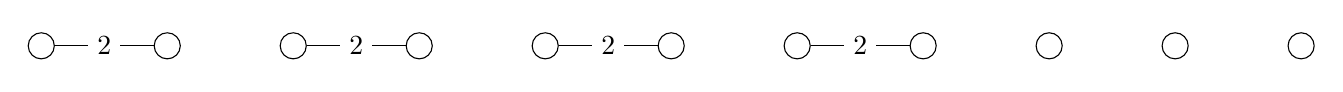
\begin{tikzpicture}[scale=.8]

        \begin{scope}[every node/.style={circle,draw}]
          \node (1)  at (-2,0)  {};
          \node (2)  at (0,0)  {};
          \node (3)  at (2,0)  {};
          \node (4)  at (4,0)  {};
          \node (5)  at (6,0)  {};
          \node (6)  at (8,0)  {};
          \node (7)  at (10,0)  {};
          \node (8)  at (12,0)  {};
          \node (9)  at (14,0)  {};
          \node (10)  at (16,0)  {};
          \node (11)  at (18,0)  {};
        \end{scope}

        \begin{scope}[every node/.style={fill=white}]

          \begin{scope}[every edge/.style={draw}]
            \path (1)  edge node {$2$} (2);
            \path (3)  edge node {$2$} (4);
            \path (5)  edge node {$2$} (6);
            \path (7)  edge node {$2$} (8);
          \end{scope}
        \end{scope}

      \end{tikzpicture}
      \caption{[1, 5, 1010, 232, 381]}
    \end{center}
  \end{figure}

\paragraph{}
If the involutions $\rho_0$ and $\rho_4$ are added to the graph, they must commute with $\rho_2$ and so the only possibilities are:
\begin{enumerate}
  \item A double edge with $\rho_2$ and link two currently fixed points.
  \item Two double edges with $\rho_2$.
  \item An alternating square with $\rho_2$.
\end{enumerate}

\paragraph{}
Since there is only one 4-transposition, there are only 12 edges to link 11 points, 2 more than the minimum. Thus if a edge is added, it must link two distinct components, expect two times. Those two edges are called "joker" edges. When an alternating square is built, one of those edge is used, it is the same if a double edge is made.

\paragraph{}
Among the three possibilites, the second is impossible because, if it is used, even once, it uses both "joker" edges and it is not possible to place the other involution.

\paragraph{}
The same choice cannot be made for $\rho_0$ and $\rho_4$. The first proposition cannot be used twice because it links two fixed points but there is only three of them and so it cannot be used two times.

\paragraph{}
If the third proposition is used twice, there are two alternating squares. If those squares does not share a vertex, they cannot be linked. Thus one square must be linked to the rest of the graph by a $\rho_1$ edge and the other by a $\rho_3$. But those two edges cannot be linked because all $\rho_2$ have already be used and no more alternating square or double edges cannot be used.

\paragraph{}
If the two squares share an edge, a $\rho_0$ and a $\rho_4$ edge are next to each other and so an alternating square must be build to solve this problem but it is impossible.

\paragraph{}
The two squares cannot share all their vertices because it will not be able to be connected two the rest of the graph.

\paragraph{}
Thus one of the involution must make an alternating square and the other must make a double edge and links two fixed points. By duality, only the case where $\rho_4$ makes an alternating square will be considered and the other doubles an edge and links two fixed points. Currently the graph is the following

\begin{figure}[H]
  \begin{center}
    \begin{tikzpicture}[scale=.8]

      \begin{scope}[every node/.style={circle,draw}]
        \node (1)  at (12,2)  {};
        \node (2)  at (12,0)  {};
        \node (3)  at (14,2)  {};
        \node (4)  at (14,0)  {};
        \node (5)  at (6,0)  {};
        \node (6)  at (4,0)  {};
        \node (7)  at (10,0)  {};
        \node (8)  at (8,0)  {};
        \node (9)  at (2,0)  {};
        \node (10) at (0,0)  {};
        \node (11) at (16,0) {};
      \end{scope}

      \begin{scope}[every node/.style={fill=white}]

        \begin{scope}[every edge/.style={draw}]
          \path (9)  edge node {$0$} (10);
          \path (7)  edge[bend right=30] node {$0$} (8);
          \path (1)  edge node {$2$} (2);
          \path (3)  edge node {$2$} (4);
          \path (5)  edge node {$2$} (6);
          \path (7)  edge[bend left=30] node {$2$} (8);
          \path (1)  edge node {$4$} (3);
          \path (2)  edge node {$4$} (4);
        \end{scope}
      \end{scope}

    \end{tikzpicture}
    \caption{The graph with only $\rho_0$ and $\rho_2$}
  \end{center}
\end{figure}

\paragraph{}
Now that all of our "joker" edges has been used, every other edge must link two different connex components of the graph.

\paragraph{}
Now the $\rho_3$ edge will be placed. It cannot be adjacent to the component consisting of the single $\rho_0$ edge or to the double edge. There are only three components that can be adjacent to such edge. Thus there are three places for two edges. But the component that we are currently builing must be linked to the rest of the graph by $\rho_1$ edges and a $\rho_1$ edge can only be connected to the single $\rho_2$ edge. This edge must so be connected by only one $\rho_3$ edge. The same applies for the fixed point that cannot be connected two times, otherwise two $\rho_3$ edges will share this vertex.

\paragraph{}
The square must thus be connected twice. There are three possibilities: the two connected vertices can be opposed or adjacent and, in this case, separated by a $\rho_1$ or a $\rho_3$ edge. This does not influence the position of the $\rho_1$ edges it is possible to continue building the graph without having to deal with cases. Here is one of the possible graphs:

\begin{figure}[H]
  \begin{center}
    \begin{tikzpicture}[scale=.8]

      \begin{scope}[every node/.style={circle,draw}]
        \node (1)  at (0,2)  {};
        \node (2)  at (0,0)  {};
        \node (3)  at (-2,2)  {};
        \node (4)  at (-2,0)  {};
        \node (5)  at (-6,0)  {};
        \node (6)  at (-4,0)  {};
        \node (7)  at (-10,0)  {};
        \node (8)  at (-8,0)  {};
        \node (9)  at (-14,0)  {};
        \node (10) at (-12,0)  {};
        \node (11) at (2,0) {};
      \end{scope}

      \begin{scope}[every node/.style={fill=white}]

        \begin{scope}[every edge/.style={draw}]
          \path (9)  edge node {$0$} (10);
          \path (7)  edge[bend right=30] node {$0$} (8);
          \path (1)  edge node {$2$} (2);
          \path (3)  edge node {$2$} (4);
          \path (5)  edge node {$2$} (6);
          \path (7)  edge[bend left=30] node {$2$} (8);
          \path (2)  edge node {$3$} (11);
          \path (4)  edge node {$3$} (6);
          \path (1)  edge node {$4$} (3);
          \path (2)  edge node {$4$} (4);
        \end{scope}
      \end{scope}

    \end{tikzpicture}
    \caption{One of the graphs after placing $\rho_3$ edges}
  \end{center}
\end{figure}

\paragraph{}
Now the two edges of $\rho_1$ must be placed, the component containing the alternating square must be attached by its left end, the one that ends with a $\rho_2$ edge. The first two component must be linked together. The first component can be attached in two ways depending on the end choosen to be attached. Here is one of the graphs:

\begin{figure}[H]
  \begin{center}
    \begin{tikzpicture}[scale=.8]

      \begin{scope}[every node/.style={circle,draw}]
        \node (1)  at (0,2)  {};
        \node (2)  at (0,0)  {};
        \node (3)  at (-2,2)  {};
        \node (4)  at (-2,0)  {};
        \node (5)  at (-6,0)  {};
        \node (6)  at (-4,0)  {};
        \node (7)  at (-10,0)  {};
        \node (8)  at (-8,0)  {};
        \node (9)  at (-14,0)  {};
        \node (10) at (-12,0)  {};
        \node (11) at (2,0) {};
      \end{scope}

      \begin{scope}[every node/.style={fill=white}]

        \begin{scope}[every edge/.style={draw}]
          \path (9)  edge node {$0$} (10);
          \path (7)  edge[bend left=30] node {$0$} (8);
          \path (5)  edge node {$1$} (8);
          \path (7)  edge node {$1$} (10);
          \path (1)  edge node {$2$} (2);
          \path (3)  edge node {$2$} (4);
          \path (5)  edge node {$2$} (6);
          \path (7)  edge[bend right=30] node {$2$} (8);
          \path (2)  edge node {$3$} (11);
          \path (4)  edge node {$3$} (6);
          \path (1)  edge node {$4$} (3);
          \path (2)  edge node {$4$} (4);
        \end{scope}
      \end{scope}

    \end{tikzpicture}
    \caption{One sggi on $A_{11}$ of rank 5}
  \end{center}
\end{figure}

\paragraph{}
There are 6 possible graphs but only one was built. The construction of the five remaining graphs is left to the reader. He can check that the graphs built match the graphs of appendix~\ref{monodromy-5}.

\end{proof}


\begin{theorem}
  None of the groups represented by the graphs of appendix~\ref{monodromy-5} are C-groups.
\end{theorem}

\begin{proof}
  By the definition of a C-group, it is sufficient to find two subsets of generators $S_1$ and $S_2$ such that $\Gamma_{S_1} \cap \Gamma_{S_2} \neq \Gamma_{S_1 \cap S_2}$.

  \paragraph{}
  In this case, they will be chosse $S_1 = \{\rho_1, \rho_2\}$ and $S_2 = \{\rho_2, \rho_3, \rho_4\}$. Here $S_1 \cap S_2 = \{\rho_2\}$ and so $\Gamma_{S_1 \cap S_2} = \Gamma_{\rho_2}$ is a cyclic group of order 2. Hence, $\rho_2$ is an involution.

  \paragraph{}
  $S_1$ will be studied more deeply, only the $\rho_1$ and $\rho_2$ edges are kept in all the possible graphs. There are only two possibles graphs:

  \begin{figure}[H]
    \begin{center}
      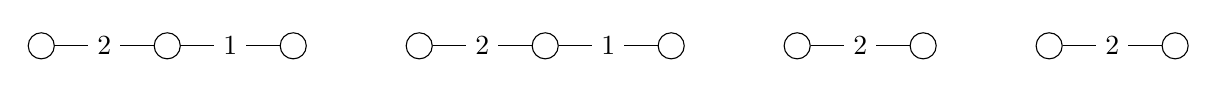
\begin{tikzpicture}[scale=.8]

        \begin{scope}[every node/.style={circle,draw}]
          \node (1)  at (-2,0)  {};
          \node (2)  at (0,0)  {};
          \node (3)  at (2,0)  {};
          \node (4)  at (8,0)  {};
          \node (5)  at (6,0)  {};
          \node (6)  at (4,0)  {};
          \node (7)  at (12,0)  {};
          \node (8)  at (10,0)  {};
          \node (9)  at (16,0)  {};
          \node (10) at (14,0)  {};
        \end{scope}

        \begin{scope}[every node/.style={fill=white}]

          \begin{scope}[every edge/.style={draw}]
            \path (2)  edge node {$1$} (3);
            \path (4)  edge node {$1$} (5);
            \path (1)  edge node {$2$} (2);
            \path (5)  edge node {$2$} (6);
            \path (7)  edge node {$2$} (8);
            \path (9)  edge node {$2$} (10);
          \end{scope}
        \end{scope}

      \end{tikzpicture}
      \caption{First possibility for $\Gamma_{S_1}$}
    \end{center}
  \end{figure}

  \begin{figure}[H]
    \begin{center}
      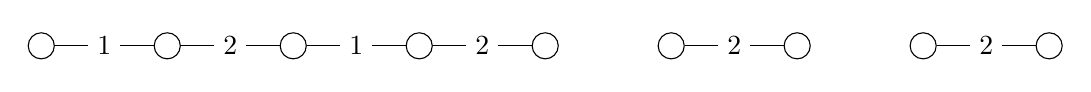
\begin{tikzpicture}[scale=.8]

        \begin{scope}[every node/.style={circle,draw}]
          \node (2)  at (0,0)  {};
          \node (3)  at (2,0)  {};
          \node (4)  at (4,0)  {};
          \node (5)  at (6,0)  {};
          \node (6)  at (8,0)  {};
          \node (7)  at (12,0)  {};
          \node (8)  at (10,0)  {};
          \node (9)  at (16,0)  {};
          \node (10) at (14,0)  {};
        \end{scope}

        \begin{scope}[every node/.style={fill=white}]

          \begin{scope}[every edge/.style={draw}]
            \path (2)  edge node {$1$} (3);
            \path (4)  edge node {$1$} (5);
            \path (3)  edge node {$2$} (4);
            \path (5)  edge node {$2$} (6);
            \path (7)  edge node {$2$} (8);
            \path (9)  edge node {$2$} (10);
          \end{scope}
        \end{scope}

      \end{tikzpicture}
      \caption{Second possibility for $\Gamma_{S_1}$}
    \end{center}
  \end{figure}

  \paragraph{}
  In the first graph, the permutation $(\rho_1 \rho_2)^2 \rho_1$ lets the points of the two isolated edges fixed because the permutation uses $\rho_2$ an even number of times. The points only linked by $\rho_1$ edges remain fixed too. But the point linked by $\rho_2$ edges in the big components are swapped. So it is possible to permute only two $\rho_2$ edges without touching the two others.

  \paragraph{}
  In the second graph, $(\rho_1\rho_2)^4 \rho_1$ gives the same result.

  \paragraph{}
  Now, let's study $S_2$, the disposition of the edges alongside the alternating square is very important. Therefore there are 3 possibilities:

  \begin{figure}[H]
    \begin{center}
      \begin{tikzpicture}[scale=.8]

        \begin{scope}[every node/.style={circle,draw}]
          \node (1)  at (-2,0)  {};
          \node (2)  at (0,0)  {};
          \node (5)  at (2,0)  {};
          \node (6)  at (4,0)  {};
          \node (7)  at (6,0)  {};
          \node (8)  at (6,2)  {};
          \node (9)  at (8,2)  {};
          \node (10) at (8,0)  {};
          \node (11) at (10,0) {};
        \end{scope}

        \begin{scope}[every node/.style={fill=white}]

          \begin{scope}[every edge/.style={draw}]
            \path (1)  edge node {$2$} (2);
            \path (5)  edge node {$2$} (6);
            \path (7)  edge node {$2$} (8);
            \path (9)  edge node {$2$} (10);
            \path (6)  edge node {$3$} (7);
            \path (10) edge node {$3$} (11);
            \path (7)  edge node {$4$} (10);
            \path (8)  edge node {$4$} (9);
          \end{scope}
        \end{scope}

      \end{tikzpicture}
      \caption{First possibility for $\Gamma_{S_2}$}
    \end{center}
  \end{figure}

  \begin{figure}[H]
    \begin{center}
      \begin{tikzpicture}[scale=.8]

        \begin{scope}[every node/.style={circle,draw}]
          \node (1)  at (-2,0)  {};
          \node (2)  at (0,0)  {};
          \node (5)  at (2,0)  {};
          \node (6)  at (4,0)  {};
          \node (7)  at (6,0)  {};
          \node (8)  at (6,2)  {};
          \node (9)  at (8,0)  {};
          \node (10) at (8,2)  {};
          \node (11) at (10,2) {};
        \end{scope}

        \begin{scope}[every node/.style={fill=white}]

          \begin{scope}[every edge/.style={draw}]
            \path (1)  edge node {$2$} (2);
            \path (5)  edge node {$2$} (6);
            \path (7)  edge node {$2$} (8);
            \path (9)  edge node {$2$} (10);
            \path (6)  edge node {$3$} (7);
            \path (10) edge node {$3$} (11);
            \path (7)  edge node {$4$} (9);
            \path (8)  edge node {$4$} (10);
          \end{scope}
        \end{scope}

      \end{tikzpicture}
      \caption{Second possibility for $\Gamma_{S_2}$}
    \end{center}
  \end{figure}

  \begin{figure}[H]
    \begin{center}
      \begin{tikzpicture}[scale=.8]

        \begin{scope}[every node/.style={circle,draw}]
          \node (1)  at (-2,0)  {};
          \node (2)  at (0,0)  {};
          \node (5)  at (2,0)  {};
          \node (6)  at (4,0)  {};
          \node (7)  at (8,2)  {};
          \node (8)  at (6,2)  {};
          \node (9)  at (6,0)  {};
          \node (10) at (8,0)  {};
          \node (11) at (10,0) {};
        \end{scope}

        \begin{scope}[every node/.style={fill=white}]

          \begin{scope}[every edge/.style={draw}]
            \path (1)  edge node {$2$} (2);
            \path (5)  edge node {$2$} (6);
            \path (7)  edge node {$2$} (8);
            \path (9)  edge node {$2$} (10);
            \path (6)  edge node {$3$} (9);
            \path (10) edge node {$3$} (11);
            \path (7)  edge node {$4$} (10);
            \path (8)  edge node {$4$} (9);
          \end{scope}
        \end{scope}

      \end{tikzpicture}
      \caption{Third possibility for $\Gamma_{S_2}$}
    \end{center}
  \end{figure}

  \paragraph{}
  The group generated by the right component is transitive because the component is connex. It's also 2-transitive, this can be checked by fixing the most right point and trying to move it's neighbor. For the first possibility this can be obtained by the permutation $\rho_2 \rho_4 \rho_3 \rho_2 \rho_3 \rho_2 \rho_3$. This can easily be proved for the three graphs and the proof is left to the reader.

  \paragraph{}
  The group is 2-transitive and thus primitive. The list of all primitive groups on seven points can be found in~\cite{buekenhout1996list}. The group is 2-transitive and so its order is a multiple of $7 \times 6 = 42$. But it is possible to find one subgroup by looking at the group generated by $\rho_2$ and $\rho_3$ only. This group is $D_{10}$ which is of order 10. The order of the group must also divides the order of those sub-groups.

  \paragraph{}
  Thus the order of the group must be a multiple of $7 \times 6 \times 5 = 210$. By looking at the list, there are only two primitive groups on 7 points such that 210 divides they orders : $A_7$ and $S_7$. But the permutation $\rho_2$ is odd on those 7 points, the only possibility is $S_7$.

  \paragraph{}
  But then every $\rho_2$ edge is an involution on those 7 points. The other component, that only contains a $\rho_2$ edge must be there to keep the parity of the whole permutation. Therefore this group contains the same involution on 4 point that was found for $\Gamma_{S_1}$. This involution is in $\Gamma_{S_1}$ and in $\Gamma_{S_2}$ but not in $\Gamma_{\rho_2}$ thus $\Gamma$ does not satisfy the intersection property and thus, is not a C-group.

\end{proof}

\paragraph{}
Now we have proven that there is no abstract polytopes of rank $5$ on $A_{11}$. Next we will prove the same for rank 4.
